\section{Design}


\subsection{Transaction Sizes}

Key points: transactions have limited size, both in space and time. A
transaction cannot take too many instructions, nor have too many memory
accesses. Of course, we're designing under an assumption about how transactions
will work... they may turn out differently. So we're designing pessimistically.

num memory accesses matter more than number of instructions, but the total length
matters too.

We can also optimize certain parts of the code with Os and other parts with
O2/3.













\begin{figure}
\centering
\hspace*{-0.3in}
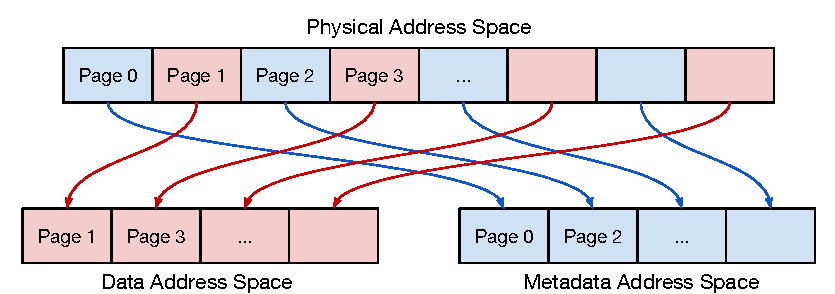
\includegraphics[width=88mm]{fig/addrspace}
\caption{Mapping the data and metadata address spaces to the physical address
space of the database file.}
\label{fig:addrspace}
\end{figure}

\begin{figure}
\centering
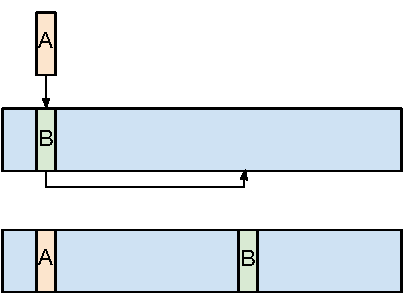
\includegraphics[width=70mm,height=50mm]{fig/cuckoo_insert}
\caption{Inserting an element that requires moving an existing element to a
partner bucket.}
\label{fig:insert}
\end{figure}

\begin{figure}
\centering
\hspace*{1mm}
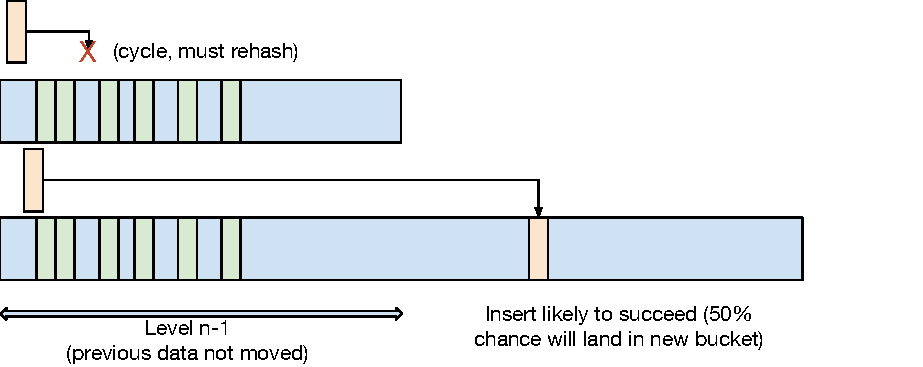
\includegraphics[width=100mm]{fig/cuckoo_rehash}
\caption{Extending the hash table to level $n$ without reinserting existing
elements. Level $n-1$ has existing elements that are not moved during the
expansion, and the newly inserted element is more than twice as likely to find
an empty bucket to insert into.}
\label{fig:rehash}
\end{figure}

